\documentclass{beamer}
\usepackage[UTF8]{ctex}
\usepackage{amsmath,amsfonts,amssymb,bm}
\usepackage{graphicx}
\usepackage{hyperref}

\title{基于标签分布感知间隔损失的\\不平衡数据学习}
\subtitle{Learning Imbalanced Datasets with Label-Distribution-Aware Margin Loss}
\author{报告人:乔彦博}
\institute{LDAM损失函数margin的推导证明}
\date{\today}

\begin{document}

\begin{frame}
    \titlepage
\end{frame}

\begin{frame}
    \centering {\LARGE 内容提要}
\vspace{1em}
\begin{flushleft}
    \tableofcontents
\end{flushleft}
\end{frame}

\section{数据不平衡学习背景}
\begin{frame}{长尾分布问题}
    % 此处建议插入图:长尾分布示意图(类别频次的长尾分布曲线)
    \begin{figure}[h]
        \centering
        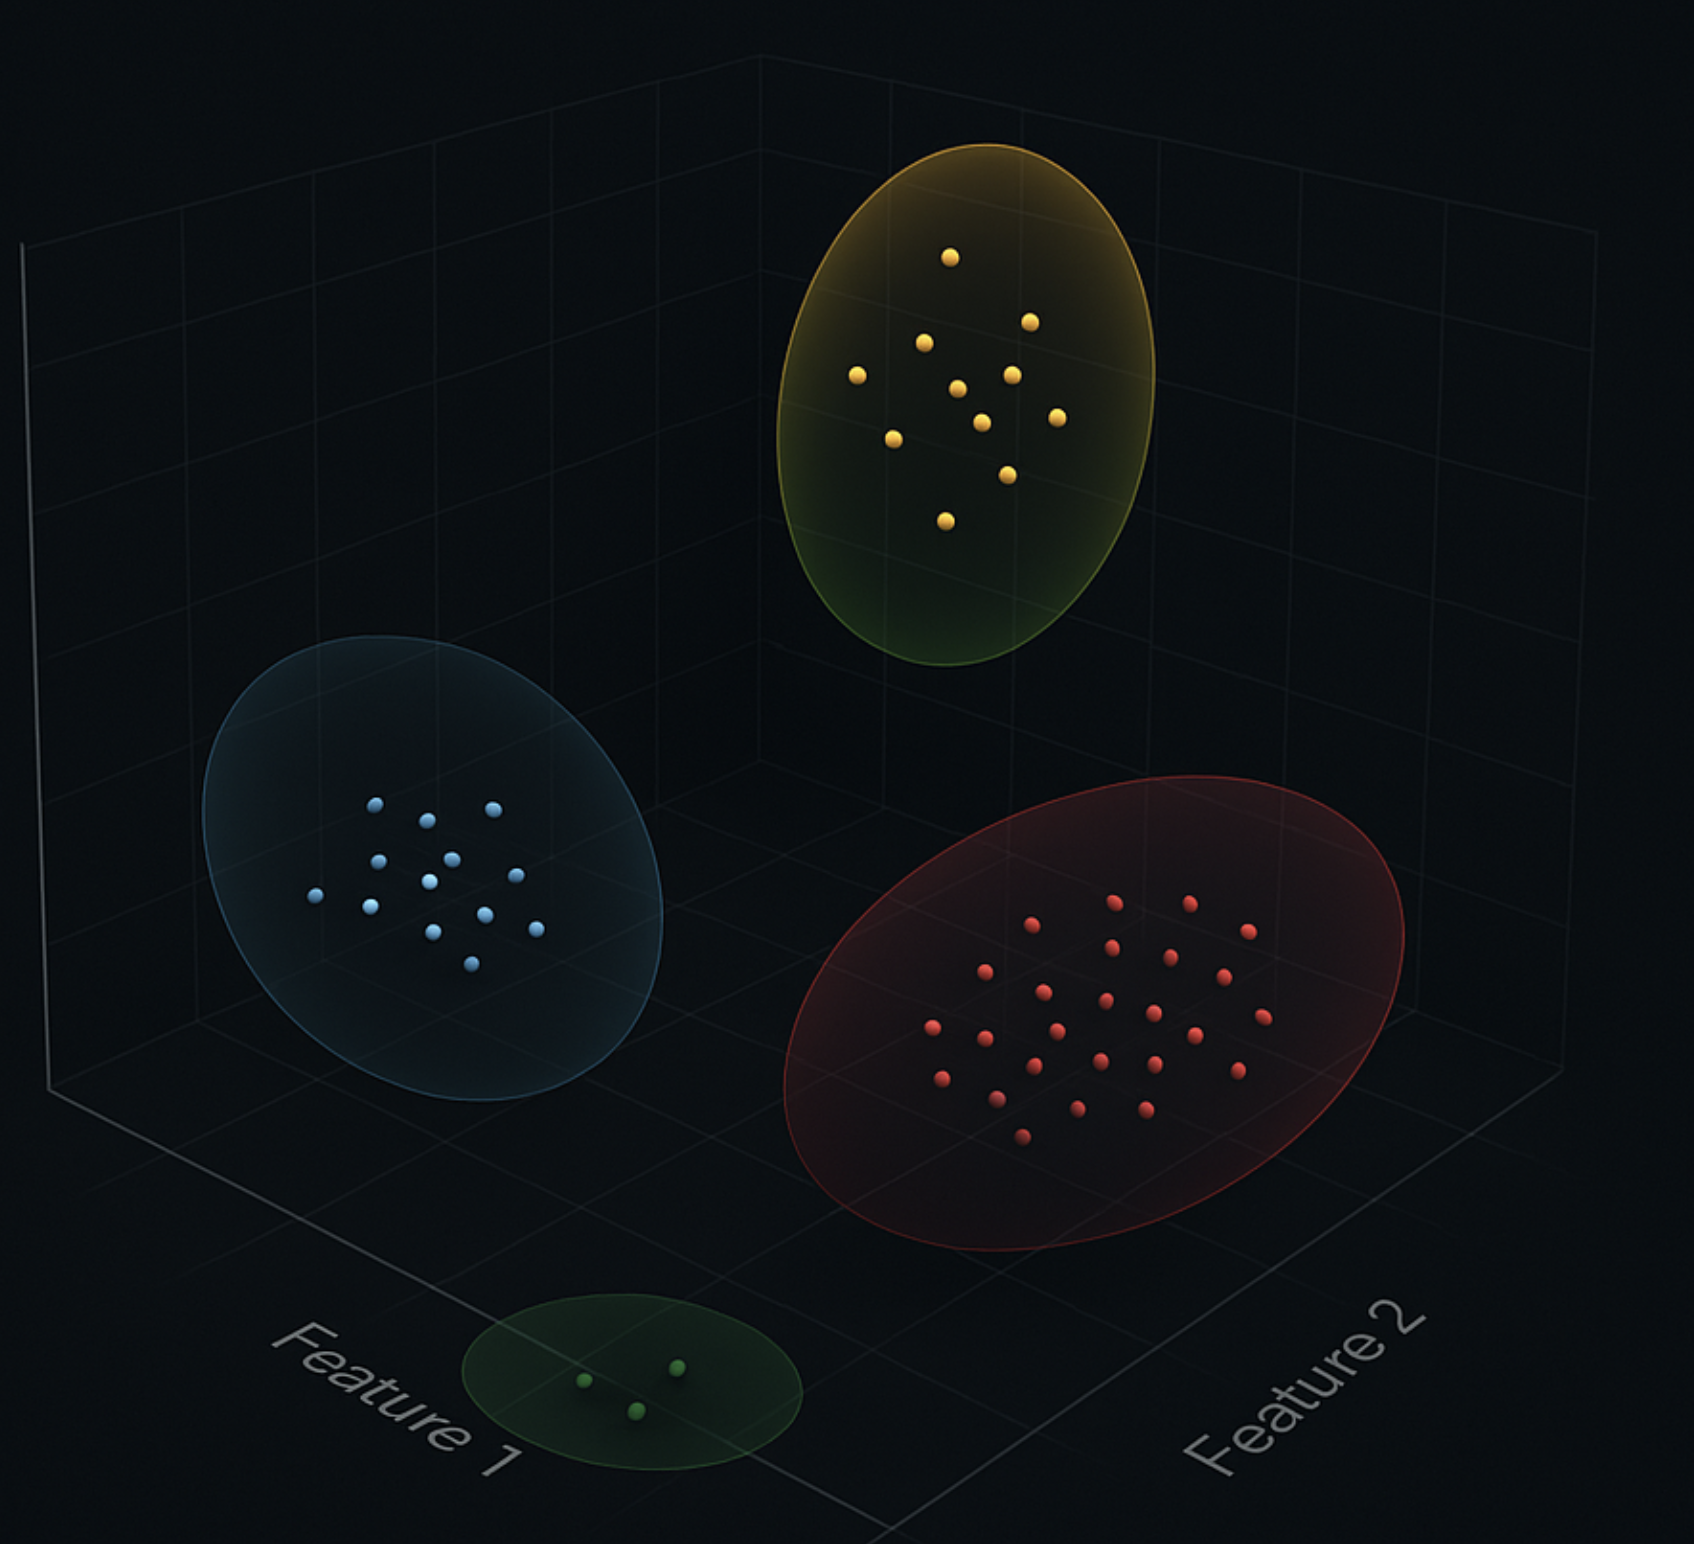
\includegraphics[width=0.7\linewidth]{long-tail.png}
        \caption{长尾分布示意图}
    \end{figure}
\end{frame}
\begin{frame}{长尾分布的训练难题}
    \begin{itemize}
        \item \textbf{长尾分布的意义}:长尾分布广泛存在于许多实际应用中,如医学的疾病影像分类中罕见病往往面临样本不足的问题,但是模型仍然需要对所有类别进行有效学习。
        \item \textbf{头部挤占空间和边界}:在长尾分布下,头部类别(样本多)在特征空间中占据主导地位,导致尾部类别(样本少)可用的判别空间被严重压缩,决策边界容易偏向头部类。
        \item \textbf{尾部样本少,难以支撑空间和间隔}:尾部类别由于样本极少,模型难以学习到稳定且具有代表性的特征,导致其决策边界不明确,分类间隔(margin)很小,泛化能力差,易被头部类误分类。
        \item 这两大难题共同导致尾部类别的准确率显著低于头部类别,是长尾分布下模型训练的核心挑战。
    \end{itemize}
\end{frame}

\begin{frame}{常规应对方法}
    \begin{itemize}
        \item \textbf{重采样(Re-sampling)}:对多数类\textbf{欠采样}或对少数类\textbf{过采样},使训练集类分布平衡。但过采样易造成少数类\textbf{过拟合},欠采样会丢失多数类信息。
        \item \textbf{重加权(Re-weighting)}:在损失函数中给予少数类样本更大权重。例如按照类别频数的倒数加权。但权重过大时训练不稳定,容易\textbf{优化困难}。
        \item 其他方法:如\textbf{特殊损失函数}(Focal Loss 等)降低易分类样本权重,或\textbf{两阶段训练}(先学特征再调分类器)等。
        \item 常规方法局限:重采样/重加权在深度网络中效果不稳(易过拟合或需精调超参),有动机探索新的不平衡学习策略。
    \end{itemize}
\end{frame}

\section{LDAM 的动机与核心思想}
\begin{frame}{LDAM 的动机与核心思想}
    \begin{itemize}
        \item \textbf{核心动机}: 少数类样本少,易过拟合,泛化误差高,需要更大的分类间隔(margin)提升鲁棒性。
        \item \textbf{关键思想}: 分类间隔应依赖类别标签,样本越少的类别,间隔应越大。
        \item \textbf{LDAM方法}: 在损失函数中引入类别相关的间隔偏移
        \[
            \Delta_j = C \cdot n_j^{-1/4}
        \]
        少数类判别要求更高置信度,提升平衡准确率。
    \end{itemize}
\end{frame}

\begin{frame}{LDAM 损失函数(交叉熵形式)}
    \begin{itemize}
        \item \textbf{平滑的交叉熵损失}: 为了优化的稳定性,LDAM 实际采用交叉熵形式加入间隔:
        \[
            L_{\text{LDAM}}(x,y) = -\log \frac{\exp(z_y - \Delta_y)}{\exp(z_y - \Delta_y) + \sum_{j \neq y}\exp(z_j)}\,,
        \] 
        其中同样 $\Delta_y = C \cdot n_y^{-1/4}$。
        \item 对正确类别的 logit 减去 $\Delta_y$,相当于提高该样本被正确分类的难度(需要更大的 logit 才有相同概率),从而有效地在概率空间实现了类依赖的间隔。
        \item 当训练集平衡时,可以视 $\Delta_y$ 取常数 $C$(不区分类别)即退化为一般的具有固定 margin 的损失【与以往工作中恒定 margin 的情况对应】。LDAM 则针对不平衡数据,动态调整 margin 大小。
        \item LDAM 通过简单修改损失函数,结合后续的训练策略(如延迟重加权),取得了优于单纯重采样/重加权的方法的效果。
    \end{itemize}
\end{frame}

% =====================  Section: 定理推导和证明  =====================
\section{定理推导和证明}

%--------------------------------
\begin{frame}{平衡误差与分类间隔}
    \begin{itemize}
        \item \textbf{平衡测试误差}  
              \[
                  L_{\text{bal}}\;=\;\frac{1}{k}\sum_{j=1}^{k} L_j,
                  \quad
                  L_j:=\Pr\!\bigl[\hat y\neq y\mid y=j\bigr].
              \]
        \item \textbf{训练硬间隔}(多分类)  
              \[
                  \gamma_j
                  \;=\;
                  \min_{x_i:y_i=j}\!\Bigl[
                     f_{y_i}(x_i)-\max_{l\neq y_i}f_l(x_i)
                  \Bigr].
              \]
        \item 理论上 $\gamma_j\!\uparrow\;\Rightarrow\;L_j\!\downarrow$  
              —— 详见后续类别级泛化界。
    \end{itemize}
\end{frame}

%--------------------------------
\begin{frame}{整体硬间隔泛化界(均衡设定回顾)}
    若模型在全部 $n$ 个样本上实现统一硬间隔 $\gamma$ 且 $\widehat L_{\gamma}=0$,则
    \[
        L_{\text{test}}
        \;\le\;
        \frac{2}{\gamma}\,\mathfrak{R}_{n}(\mathcal{F})
        +\sqrt{\frac{\ln(2/\delta)}{2n}}
        \;\lesssim\;
        \frac{C(\mathcal F)}{\gamma\sqrt n},
        \quad
        \text{(概率} \;1-\delta\text{)}.
    \]
    该结果来自 Rademacher 复杂度泛化界,说明
    \(
        L_{\text{test}}
        =O\!\bigl(\gamma^{-1}n^{-1/2}\bigr).
    \)
    \vskip2mm
    \textbf{局限:} 最小 $\gamma$ 往往由多数类决定,无法刻画类别不平衡。
\end{frame}

%--------------------------------
\begin{frame}{类别级硬间隔泛化界(定理 \ref{thm:class})}
    对于类别 $j$,若 $\widehat L_{\gamma_j,j}=0$,则以概率 $1-\delta$:
    \[
        L_j
        \;\le\;
        \frac{2}{\gamma_j}\,\mathfrak{R}_{n_j}(\mathcal F)
        +\sqrt{\frac{\ln(2/\delta)}{2n_j}}
        \;\lesssim\;
        \frac{C_1}{\gamma_j}\sqrt{\frac{C(\mathcal F)}{n_j}}
        +\frac{1}{\sqrt{n_j}}.
    \]
    \begin{itemize}
        \item 首项支配:$\displaystyle L_j=O\!\bigl(\gamma_j^{-1}n_j^{-1/2}\bigr)$。
        \item $n_j$ 小的类别需更大 $\gamma_j$ 才能保持同等误差。
    \end{itemize}
\end{frame}

%--------------------------------
\begin{frame}{平衡误差上界}
    平均各类界得
    \[
        L_{\text{bal}}
        \;\le\;
        \frac{C_1}{k}\sum_{j=1}^{k}
        \frac{1}{\gamma_j}\sqrt{\frac{C(\mathcal F)}{n_j}}
        +\frac{1}{k}\sum_{j=1}^{k}\!\frac{1}{\sqrt{n_j}}
        \;\approx\;
        \color{blue}{\frac{C'}{k}\sum_{j=1}^{k}\frac{1}{\gamma_j\sqrt{n_j}}}.
    \]
    \textbf{结论:} 最主要的误差来源是  
    \(
       \displaystyle\sum_{j} 1/\!\bigl(\gamma_j\sqrt{n_j}\bigr).
    \)
\end{frame}

%--------------------------------
\begin{frame}{二分类最优间隔分配}
    \[
        \min_{\gamma_1,\gamma_2>0}
        \frac{1}{\gamma_1\sqrt{n_1}}
        +\frac{1}{\gamma_2\sqrt{n_2}}
        \quad
        \text{s.t.}\;
        \gamma_1+\gamma_2=\beta.
    \]
    \begin{enumerate}
        \item 拉格朗日函数  
              $\displaystyle 
              \mathcal{L}=\frac{1}{\gamma_1\sqrt{n_1}}
              +\frac{1}{\gamma_2\sqrt{n_2}}
              +\lambda(\gamma_1+\gamma_2-\beta)$。
        \item 导数置零  
              $\partial_{\gamma_j}\mathcal L=0
              \;\Rightarrow\;
              \gamma_j^2\sqrt{n_j}=1/\lambda$。
        \item 比值关系  
              $\displaystyle
              \frac{\gamma_1}{\gamma_2}=\bigl(n_2/n_1\bigr)^{1/4}$。
    \end{enumerate}
    \[
        \therefore\quad
        \boxed{\gamma_j\propto n_j^{-1/4}}\quad(j=1,2).
    \]
\end{frame}

%--------------------------------
%----------- Page 1 -----------
\begin{frame}[fragile]{多分类最优间隔定理}
\begin{theorem}[多分类最优间隔]
在 $k$ 分类问题中,若假设间隔预算约束
\(\sum_{j=1}^k \gamma_j = M\),则最小化
\(\sum_{j=1}^k \frac{1}{\gamma_j\sqrt{n_j}}\)
的最优解满足
\[
\gamma_j \;\propto\; n_j^{-1/4},
\quad j=1,\dots,k.
\]
\end{theorem}
\end{frame}

%----------- Page 2 -----------
\begin{frame}[fragile]{多分类最优间隔定理——证明}
\begin{proof}
同样以拉格朗日乘子法处理
\[
\mathcal{L}
= \sum_{j=1}^k \frac{1}{\gamma_j\sqrt{n_j}}
+ \lambda\Bigl(\sum_{j=1}^k\gamma_j - M\Bigr).
\]
对每个 $\gamma_j$ 求偏导:
\[
-\frac{1}{\gamma_j^{2}\sqrt{n_j}} + \lambda = 0
\;\Longrightarrow\;
\gamma_j^2\sqrt{n_j} = \frac{1}{\lambda} = \text{const}.
\]
由此得 $\gamma_j\propto n_j^{-1/4}$。
\end{proof}
\end{frame}


%--------------------------------
\begin{frame}{LDAM 损失的理论支撑}
    \begin{itemize}
        \item LDAM 设置类别偏移  
              $\displaystyle \Delta_j=C\cdot n_j^{-1/4}$,
              与最优间隔 $\gamma_j\!\propto\! n_j^{-1/4}$ 完全一致。
        \item 在 \emph{慢速率}($L_j\sim n_j^{-1/2}$)下指数为 $-1/4$。  
              若达到 \emph{快速率}($L_j\sim n_j^{-1}$)则推导得 $-1/3$,  
              但经验上 $-1/4$ 更稳健。
        \item 因此 LDAM 近似最优地平衡了不平衡数据集的各类泛化误差。
    \end{itemize}
\end{frame}
%=====================================================================

\section{个人工作和改进}

\begin{frame}{尝试过的改进和效果}
    在本篇论文的基础上,我尝试了下面的改进和变体:
    \begin{itemize}
        \item \textbf{模型的融合}: 尝试在训练的最后阶段保存多个checkpoint,最后检测互补的匹配程度,进行模型融合。结果发现融合后的模型在少数类上有一定提升,但整体效果有限。将模型准确度从41.7\%提升至了42.1\%。
        \item \textbf{后训练微调}: 在训练结束后,使用少数类样本进行微调(效果最差的20个类使用40\%的训练样本)。将模型准确率提升至43.84\%。
        \item \textbf{尝试引用其他的损失函数}: 通过调研和搜索,我发现了长尾学习领域在表征层的表征能力和分类层的训练上有不同的见解,注意到PaCo(2021)这篇论文提出的\textbf{对比学习}方法,将模型准确率提升到了要求的50\%以上。
    \end{itemize}
\end{frame}

\begin{frame}{LDAM和PaCo的融合改进策略}
    \begin{itemize}
        \item \textbf{LDAM与PaCo的结合}: 在LDAM的基础上,结合PaCo的对比学习思想,设计了一个新的损失函数。该函数在分类层引入了对比损失,使得同类样本之间的距离更近,不同类样本之间的距离更远。
        \item \textbf{实验结果}: 经过实验验证,这种结合方法在少数类样本上表现出更好的鲁棒性和泛化能力。模型准确率提升至了55\%。
        \item \textbf{未来工作}: 计划进一步优化对比损失的设计,并探索更多类别不平衡问题的解决方案。
    \end{itemize}
\end{frame}

\section{结论与讨论}
\begin{frame}{结论与讨论}
    \begin{itemize}
        \item \textbf{总结}: LDAM 方法,其通过赋予少数类更大的分类间隔来提升不平衡数据集的整体性能。LDAM损失在理论上有泛化误差界的支撑,证明了按 $n_j^{-1/4}$ 规模调整间隔的合理性。
        \item \textbf{实践建议}: LDAM 实现简洁、易与现有训练流程结合。论文中作者采用\textbf{延迟重加权}(先用 LDAM 进行标准训练,再在后期降低学习率的阶段引入类别权重)策略取得最佳效果。调参方面,间隔系数 $C$ 可通过验证集调整,一般少数类需要显著但不过大的 margin。
        \item \textbf{与重采样/重加权关系}: LDAM 提供了一种\textbf{替代思路},直接从决策函数角度调整模型对不同类别的区分裕度,而非仅调整样本权重。实际上,LDAM 在二分类情形下相当于调整判决阈值,使少数类要求更高置信度,类似于一种\textbf{隐式重加权}。LDAM 可与采样/加权结合使用:先用 LDAM 获取良好特征,再施加轻量的重加权微调,以进一步平衡性能。
        \item LDAM 的思想对不平衡学习具有启发性:通过增加margin,提高少数类边界的鲁棒性,兼顾了模型泛化能力与易优化性,为类别不平衡问题提供了新的解决范式。
    \end{itemize}
\end{frame}

\end{document}
